\chapter{Pilots}
\section{First pilot: feedback and results}
We launched Reminisce.me to the public and asked family and friends to play the game. Over the course of roughly one week people have answered 1227 over the course of 83 games. We had 25 users which brings us to an average of 3.32 games played by user.
\subsection{Selected Questions}
During this trial, people answered 377 order questions, 348 timeline questions, 317 multiple choice questions and 185 geolocation questions. Of those questions 159 order questions, 174 timeline questions, 192 multiple choice questions and 158 geolocation questions were correct.\\
An other interesting statistics is the number of avoided questions. Without taking into account the state of the board, one can see that 407 order questions, 502 timeline questions, 443 multiple choice questions and 142 geolocation questions were not answered. Aside from random factors (such as the position of the board, which questions were locked etc...), this statistics can be explained by two main factors: the fun of playing a certain question type and the perceived difficulty. While there is nothing that can be said about order question (the number of answered ones is close to the number of avoided ones), it seems like people have a tendency to avoid timeline and multiple choice questions and based on the feedback we got from the users, it might be linked to the perceived difficulty. On the other hand the geolocation are picked with a visibly high ratio. The high success rate on this kind of question is probably a good explanation. Figure \ref{fig:p1TotCorrectAvoid} shows a summary of those results.
\begin{figure}
\centering
{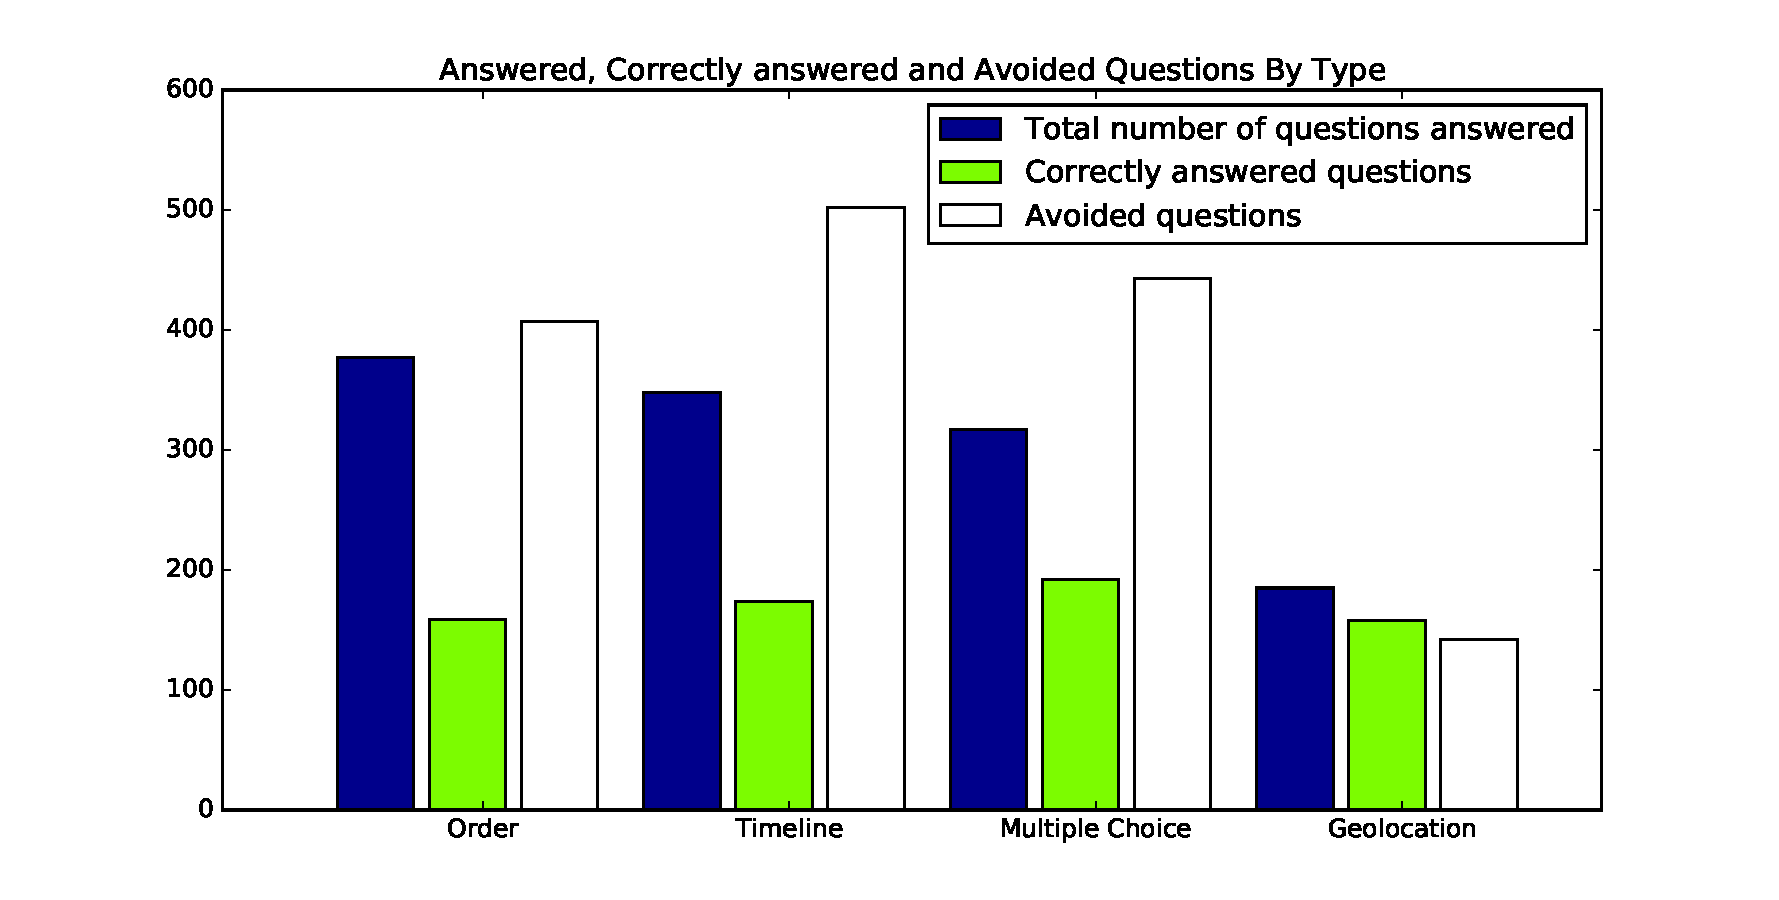
\includegraphics[width=4in]{images/pilot_1_selected_questions.pdf}}
\caption{Total, Correct and Avoided Questions Answered By Type}
\label{fig:p1TotCorrectAvoid}
\end{figure}
\subsection{Remembered Or Randomly Selected}
As for the pilot in June 2016, we can conclude that on average the players tend to try and remember the anwers. The average performance for ordering questions was 35.04\% success rate while when answering at random would yield a 16.67\% success. For timeline we get a 51.07\% success which is more than the 33.33\% random success rate. The result is the same for the multiple choice questions with respectively 58.6\% and 25\% for the measured and random success rate. Finally we measured an extraordinary 61.5\% average success rate on the geolocation. While this last result is impressive it came with a rather high standard deviation and, given the low number of geolocalised posts, the amount of different questions is low and most of the players would be able to learn the answers by heart. Figure \ref{fig:p1Correct} shows a summary of those results.\\
The high variance makes it hard to see how most of the users behaved. The box plot shown on figure \ref{fig:p1Boxes} tells us that for the timeline questions, more than 75\% of users were better than random and that half of the user had between 40\% and 60\% success, which approximatively what we wish to achieve with the difficulty in the second pilot. For order questions, more than half of the participants were better than random but most of the users had a success rate between 15\% and 51\% which is way too low so we would expect the difficulty to improve those results. The multiple choice results give that more than 75\% of the players were better than the random choice and for most of the people the average success rate was between 45\% and 75\%. This is a bit too high and we would expect that the implementation of difficulty would reduce that. When it comes to the geolocation questions we run into some issues, most of the people who had some of them had a success rate between 90\% and 100\%, this corroborates the hypothesis that most of the people who have this kind of question have so few that they can memorize them.
\begin{figure}
\centering
{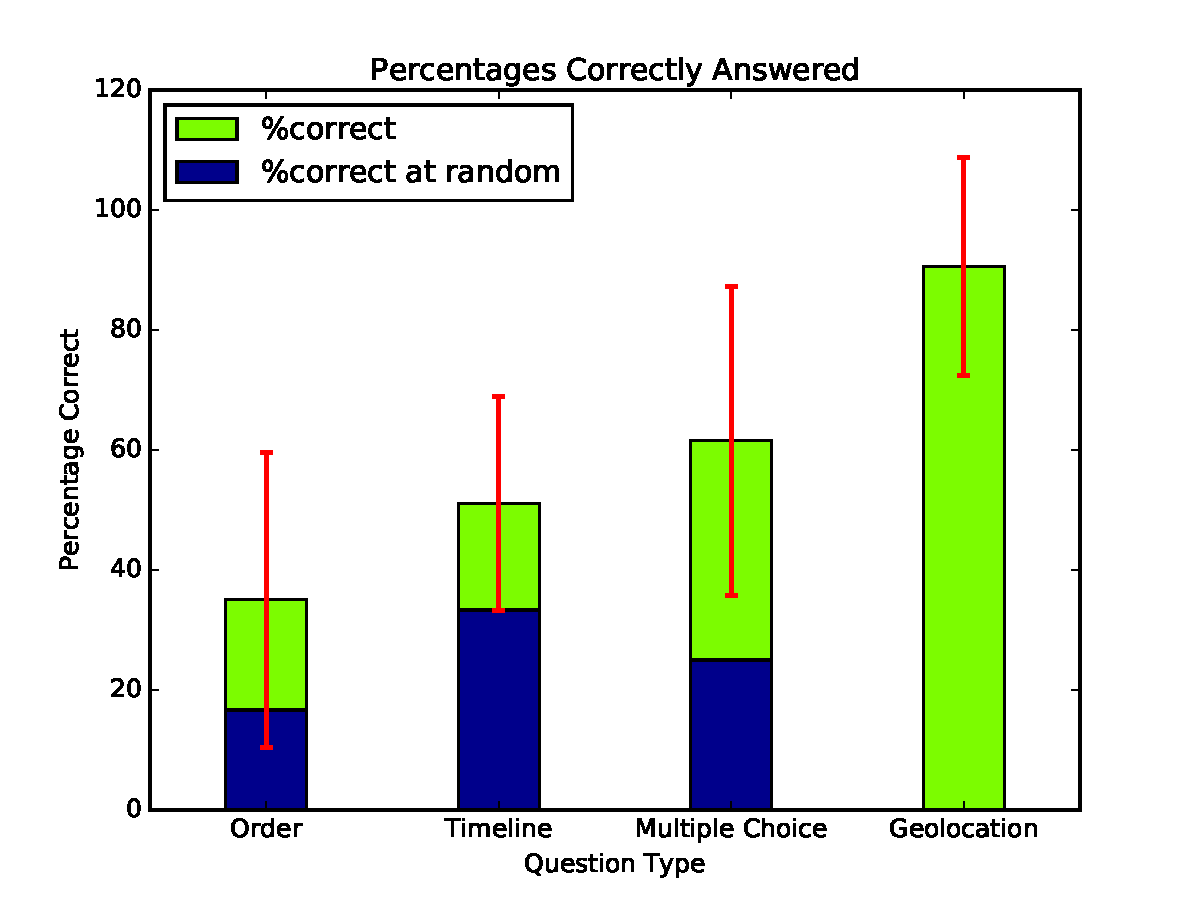
\includegraphics[width=4in]{images/pilot_1_correct.pdf}}
\caption{Percentages Correctly Answered}
\label{fig:p1Correct}
\end{figure}
\begin{figure}
\centering
{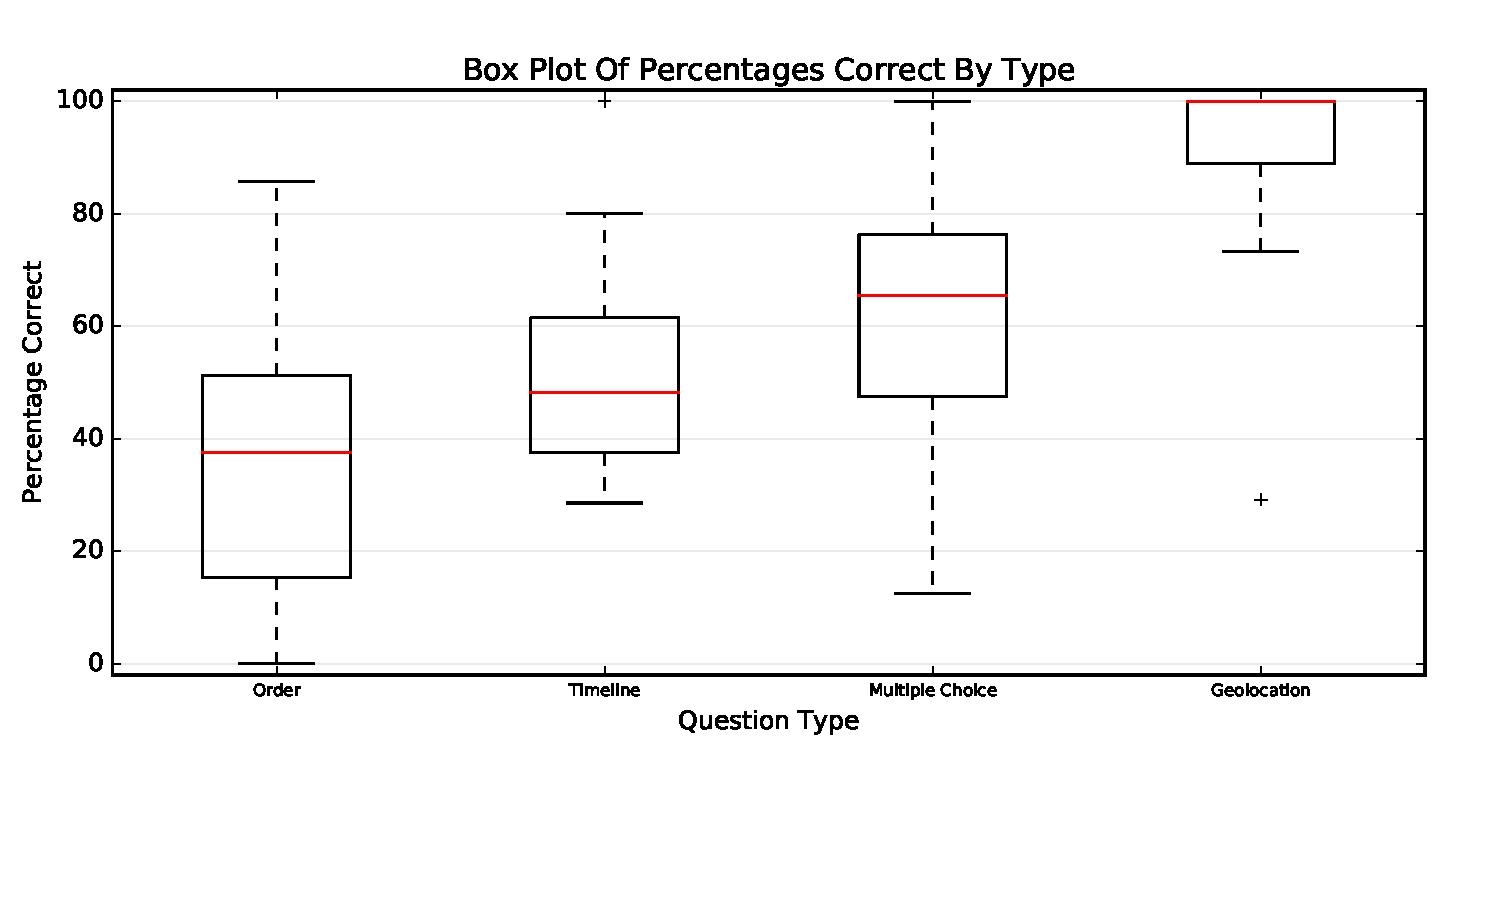
\includegraphics[width=4in]{images/pilot_1_boxplot.pdf}}
\caption{Percentages Correctly Answered Box Plots}
\label{fig:p1Boxes}
\end{figure}

\section{Time spent}
Figure \ref{fig:p1BoxesTime} shows that the time spent on timeline and multiple choice questions is pretty similar, it is a little higher for the multiple choice questions which can be explained by the higher number of possible answers. The ordering questions take more time probably because of the time taken for dragging the items. The most time is spent on the geolocation questions, it seems that there is some more thinking and the players might also be slowed down by the time taken to type their answer. However, it does not indicate that remembering a place is harder as the success rate on this kind of question is really high.
\begin{figure}
\centering
{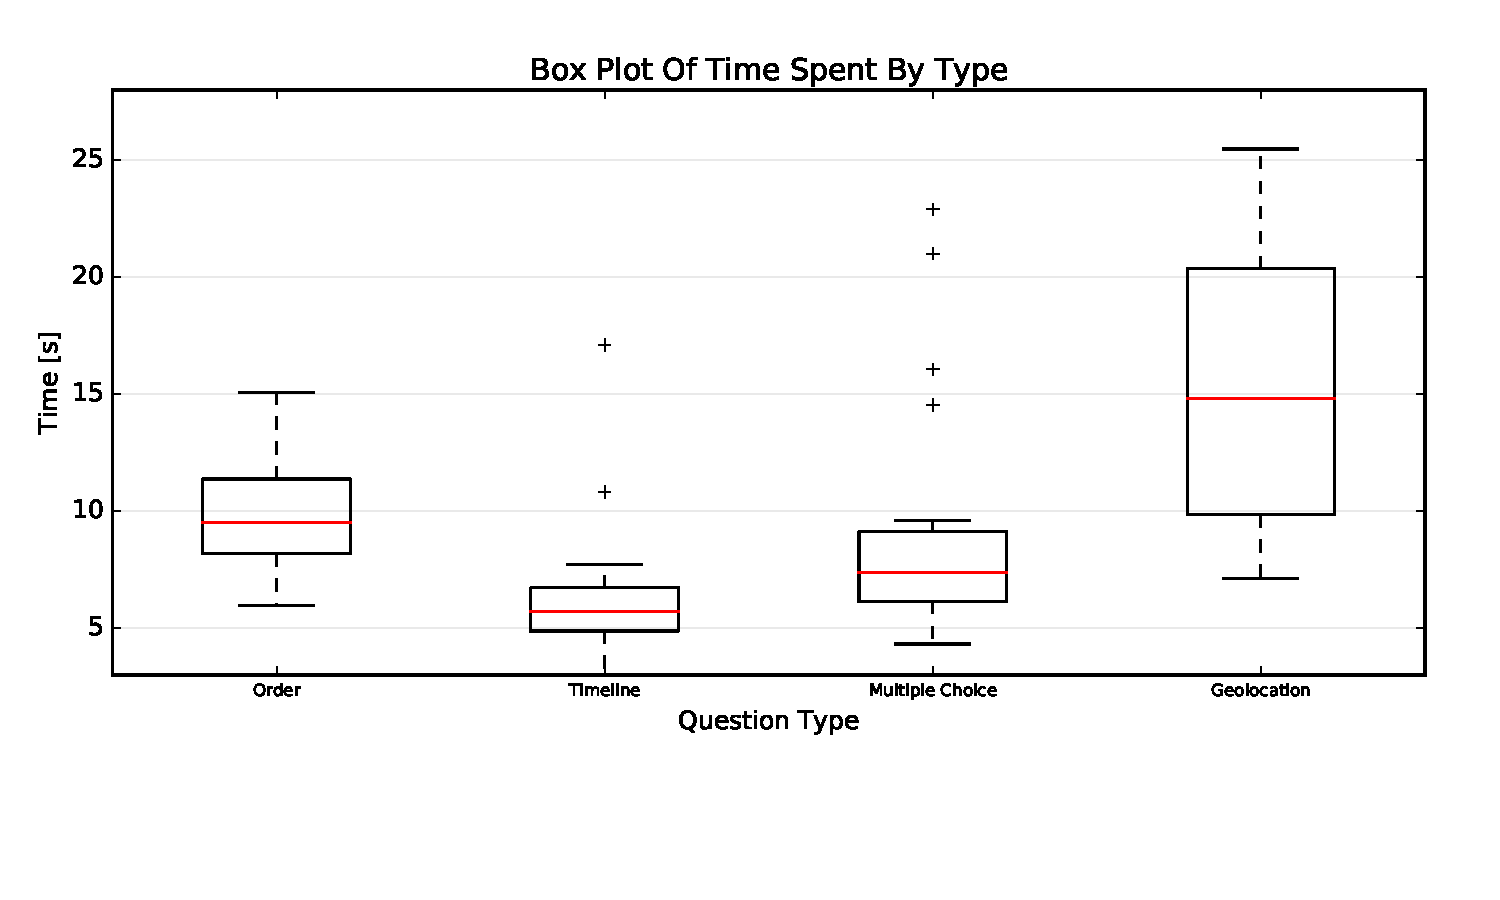
\includegraphics[width=4in]{images/pilot_1_boxplot_time.pdf}}
\caption{Box Plots Of Time Spent By Type}
\label{fig:p1BoxesTime}
\end{figure}

\section{Second pilot: on the influence of difficulty}